\documentclass[10pt,dvipdfmx]{jsarticle}
\usepackage{ascmac}
\usepackage[margin=15truemm]{geometry}
\usepackage{amsmath}
\usepackage[dvipdfmx]{graphicx}
\usepackage{subcaption}
\setlength{\columnseprule}{0.3mm}


\begin{document}

\title{信号処理特論 第11回課題}
\author{視覚認知システム研究室\\学籍番号:2433730032 岡村 翼}
\date{\today}
\maketitle

{\textgt{課題} }
配布したプリントをよく読んでDFTおよびIDFTに関して理解を深めた後、\\
(1)各自の研究に関するデータ(信号)について、信号をDFTし、実部・虚部、振幅スペクトル・位相スペクトルを求める.\\
(2)各自の信号をDFTした結果にIDFTを適用し、元の信号に戻ることを確認する.\\
(3)DFT, IDFTプログラム、原信号、DFTの実部・虚部、振幅スペクトル・位相スペクトル、そしてIDFTして元に戻った波形のグラフ(グラフは計6つ)、そして簡単な考察をまとめてレポートにする。\\

ある動画中の人物検出モデルが検出した鼻のx座標をサンプルとして用いた。\\
以下に課題について出力したグラフを示す。\\
動画中の鼻のx座標は、人物がカメラに対して左右に動いた時に変動する。
位相スペクトルから0.1から0.4にかけて位相差が少ない。
  \begin{figure}[h]
    \centering
\begin{subfigure}[b]{0.45\textwidth}
      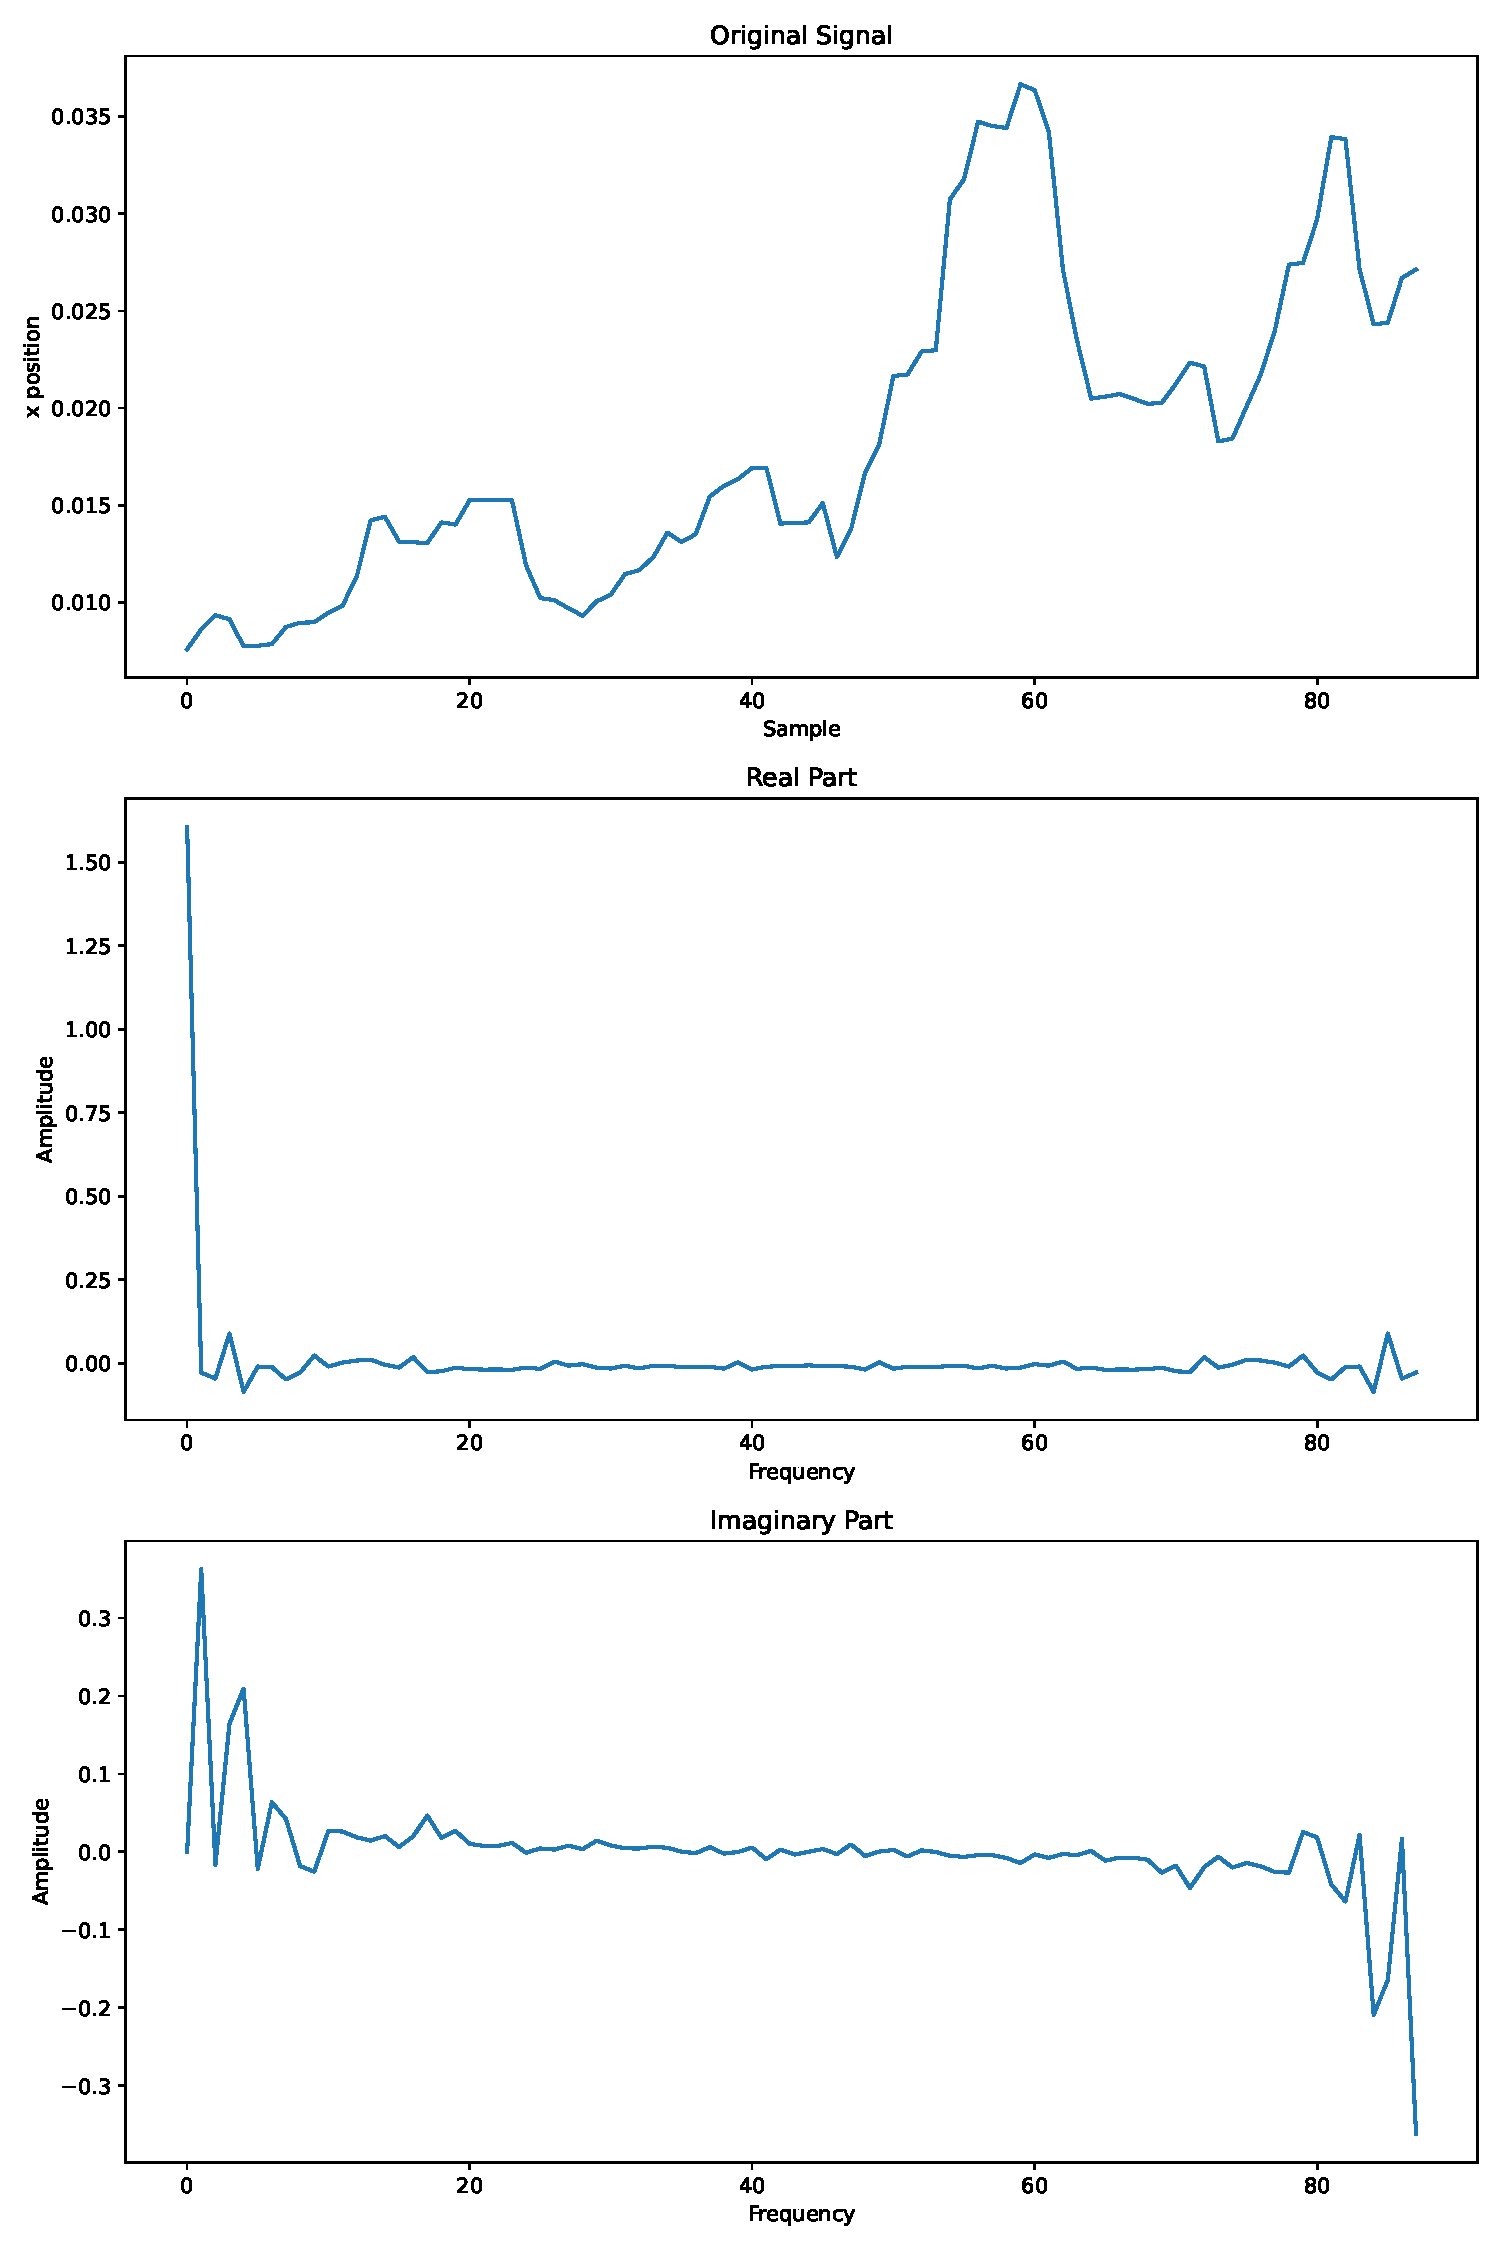
\includegraphics[width=0.8\textwidth]{DFT1.pdf}
      \label{1}
\end{subfigure}
\begin{subfigure}[b]{0.45\textwidth}
      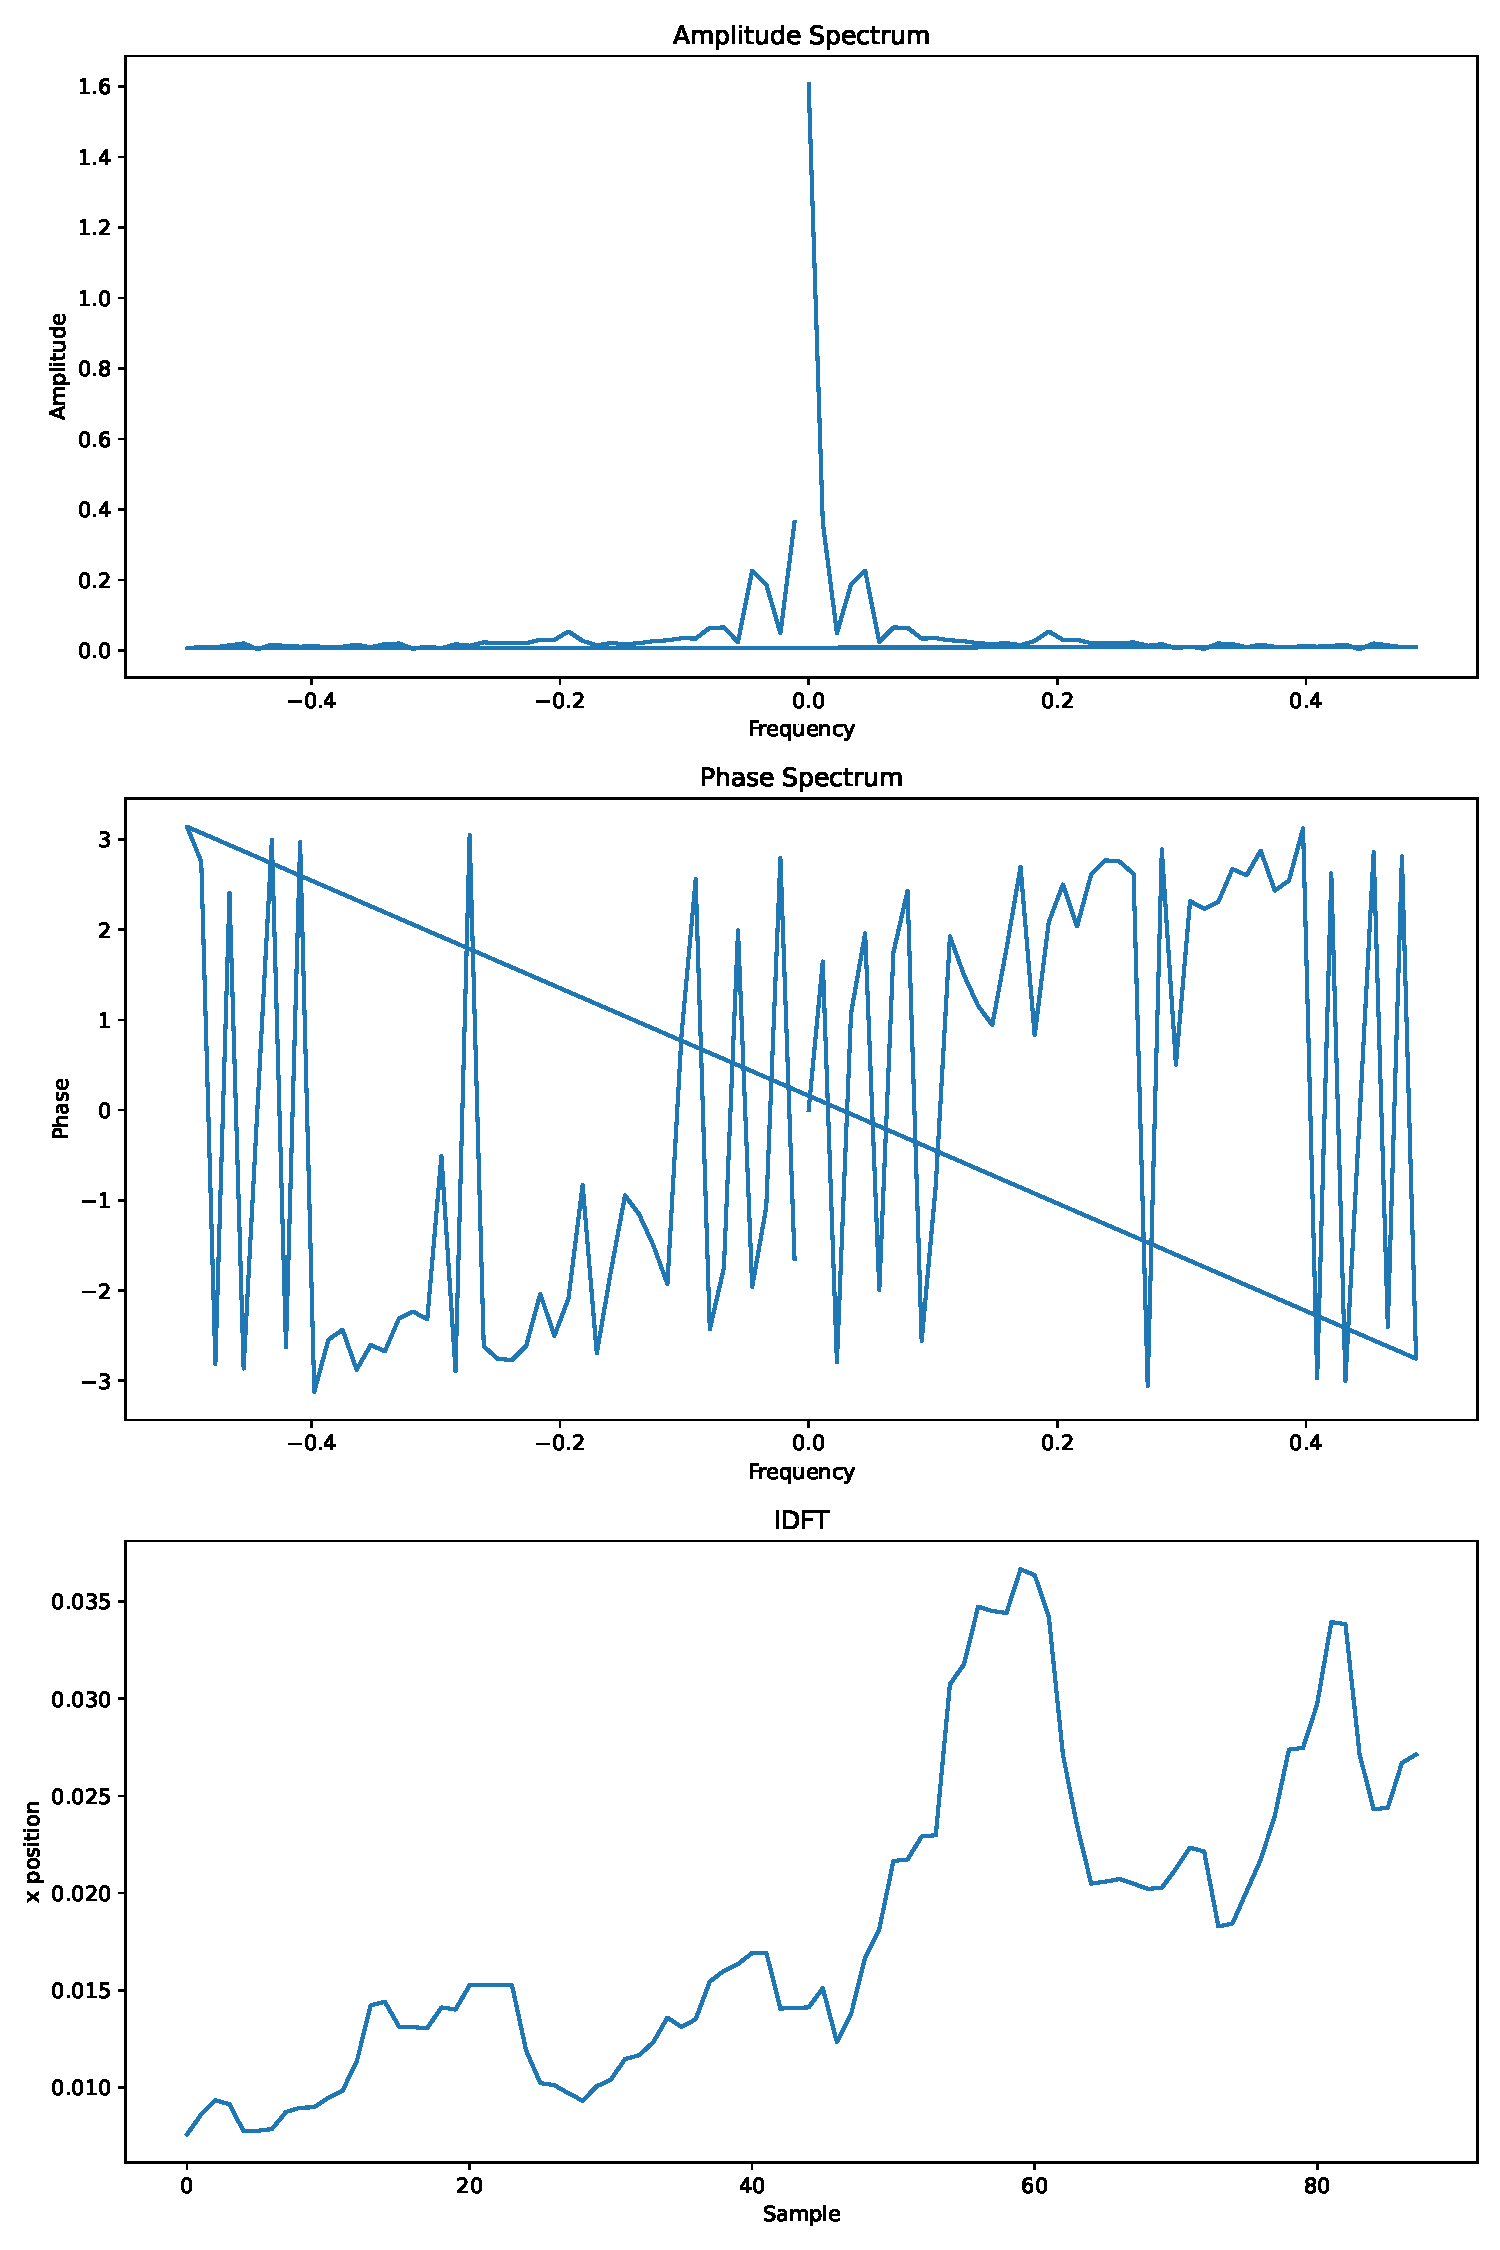
\includegraphics[width=0.8\textwidth]{DFT2.pdf}
      \label{2}
\end{subfigure}
 \end{figure}
\end{document}